% 建议使用 XeLaTeX 或 LuaLaTeX 编译(中文与公式支持更佳)
\documentclass[UTF8,zihao=-4]{ctexart}

\usepackage[a4paper,margin=2.5cm]{geometry}
\usepackage{amsmath, amssymb, amsthm}
\usepackage{bm}
\usepackage{hyperref}
\usepackage{graphicx}
\usepackage{caption}
\usepackage{listings}
\usepackage{xcolor}
\usepackage{float}
\usepackage{placeins}
\graphicspath{{figures/}}

\lstdefinestyle{code}{
  basicstyle=\ttfamily\small,
  numbers=left,
  numberstyle=\tiny,
  numbersep=8pt,
  keywordstyle=\color{blue},
  commentstyle=\color{teal!70!black},
  stringstyle=\color{orange!70!black},
  showstringspaces=false,
  breaklines=true,
  frame=single,
  framerule=0.3pt,
  rulecolor=\color{black!15}
}
\lstset{style=code}

\title{深度 Q 网络(DQN):原理、公式、应用与实战}
\author{}
\date{\today}

\begin{document}
\maketitle

\section{引言}
深度 Q 网络(Deep Q-Network, DQN)利用深度神经网络近似最优动作价值函数,并通过经验回放与目标网络稳定训练,使强化学习能处理像素级复杂输入。DQN 是深度强化学习迈向高维任务的里程碑。

\section{原理与公式}
\subsection{价值函数逼近}
设在线网络 \(Q_\theta(s,a)\) 与目标网络 \(Q_{\theta^-}(s,a)\),对转移 \((s,a,r,s')\) 的平方 TD 损失为:
\begin{equation}
L(\theta) = \big( r + \gamma \max_{a'} Q_{\theta^-}(s',a') - Q_\theta(s,a) \big)^2.
\end{equation}
通过从回放缓存 \(\mathcal{D}\) 抽样小批量进行梯度下降。

\subsection{目标网络更新}
目标网络参数周期性或通过 Polyak 平均更新:
\begin{equation}
\theta^- \leftarrow \tau \theta + (1-\tau) \theta^-.
\end{equation}
缓慢移动的目标缓解了估计震荡问题。

\subsection{经验回放}
交互产生的转移存入回放缓存,随机抽样打破时序相关性,提高样本利用率。优先级回放则根据 TD 误差加权采样,进一步提升效率。

\section{应用与技巧}
\begin{itemize}
  \item \textbf{Atari 游戏}:DQN 首次实现像素输入下的超人类表现。
  \item \textbf{机器人与仿真}:离散化动作控制任务。
  \item \textbf{运营优化}:对复杂状态进行决策优化。
  \item \textbf{实用建议}:输入规范化、奖励裁剪、探索率衰减、监控损失和 TD 误差,并使用梯度裁剪保证稳定。
\end{itemize}

\section{Python 实战}
脚本 \texttt{gen\_dqn\_figures.py} 在一维连续状态离散动作任务上训练简化 DQN,记录回报曲线与学到的状态-动作价值热力图。
\begin{lstlisting}[language=Python,caption={脚本 gen_dqn_figures.py 片段}]
q_target = reward + gamma * np.max(target_network(next_state), axis=0)
q_values = online_network(state)
loss = mse(q_target, q_values[action])
optimizer.zero_grad(); loss.backward(); optimizer.step()
\end{lstlisting}

\section{实验结果}
\begin{figure}[H]
  \centering
  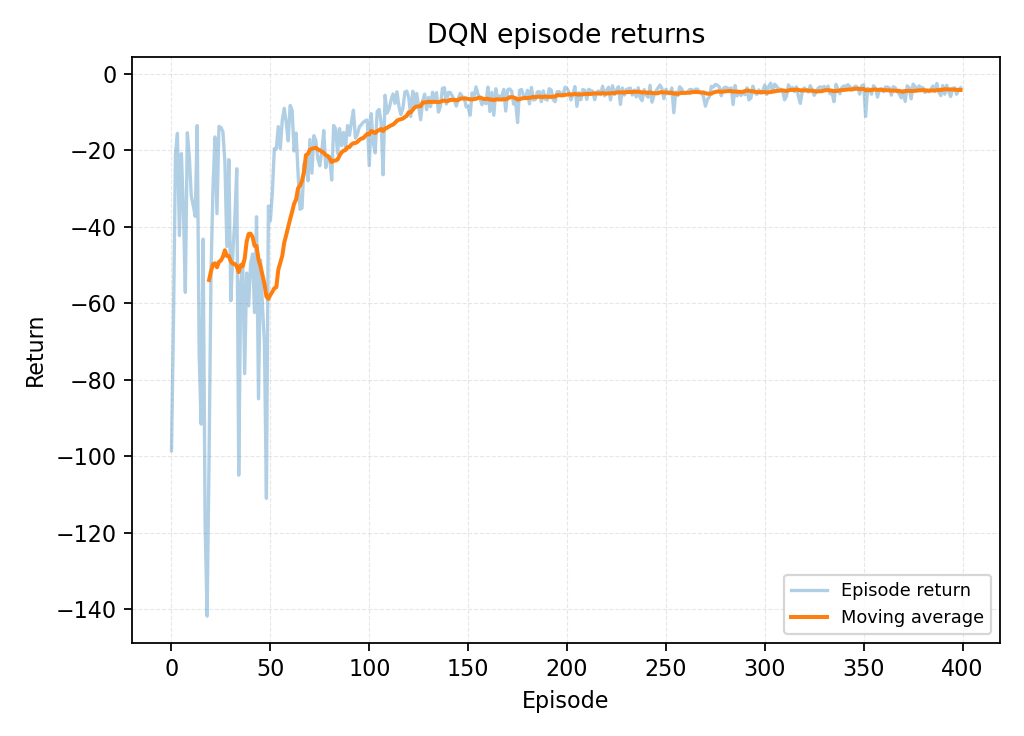
\includegraphics[width=0.8\linewidth]{dqn_returns.png}
  \caption{DQN 训练过程中的回报收敛趋势}
  \label{fig:dqn_returns_cn}
\end{figure}

\begin{figure}[H]
  \centering
  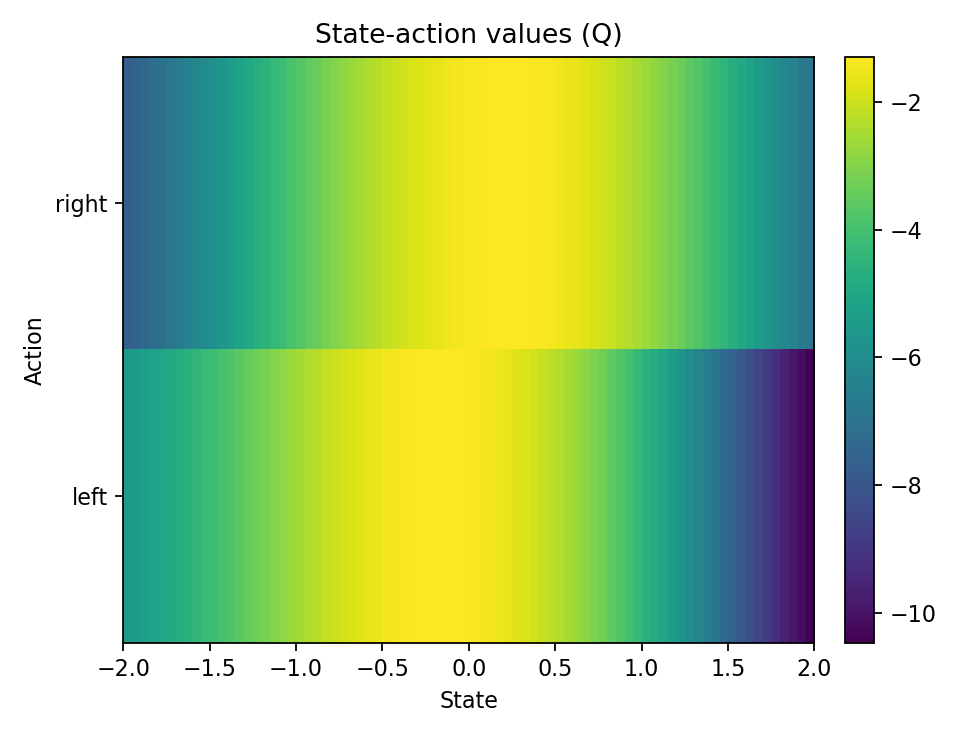
\includegraphics[width=0.82\linewidth]{dqn_q_values.png}
  \caption{学到的状态-动作价值热力图,展示最优策略偏好}
  \label{fig:dqn_q_values_cn}
\end{figure}

\FloatBarrier
\section{总结}
DQN 通过经验回放与目标网络稳定深度价值学习,适合高维离散动作任务。合理调节学习率、探索率与更新策略是收敛关键。示例说明回报不断提升,且 Q 值热力图反映最优行动偏好。

\end{document}